In diesem Versuch nutzen wir eine Quecksilber-Franck-Hertz-Röhre um verschiedene Effekte zu untersuchen.
\section{Aufbau}
Als erstes bauen wir den Versuch wie in Aufgabenstellung und Hilfe beschrieben auf.
\section{Bestimmung der Kontaktspannung zwischen Kathode und Anode}
Dann ermitteln wir die Thermokontaktspannung. Bei der Aufnahme der Daten haben wir leider Versäumt den Graphen der Messung bei 120$\; ^\circ $C abzuspeichern, weswegen für diesen nur die Daten ohne Bild vorliegen.
\begin{figure}
	\centering
	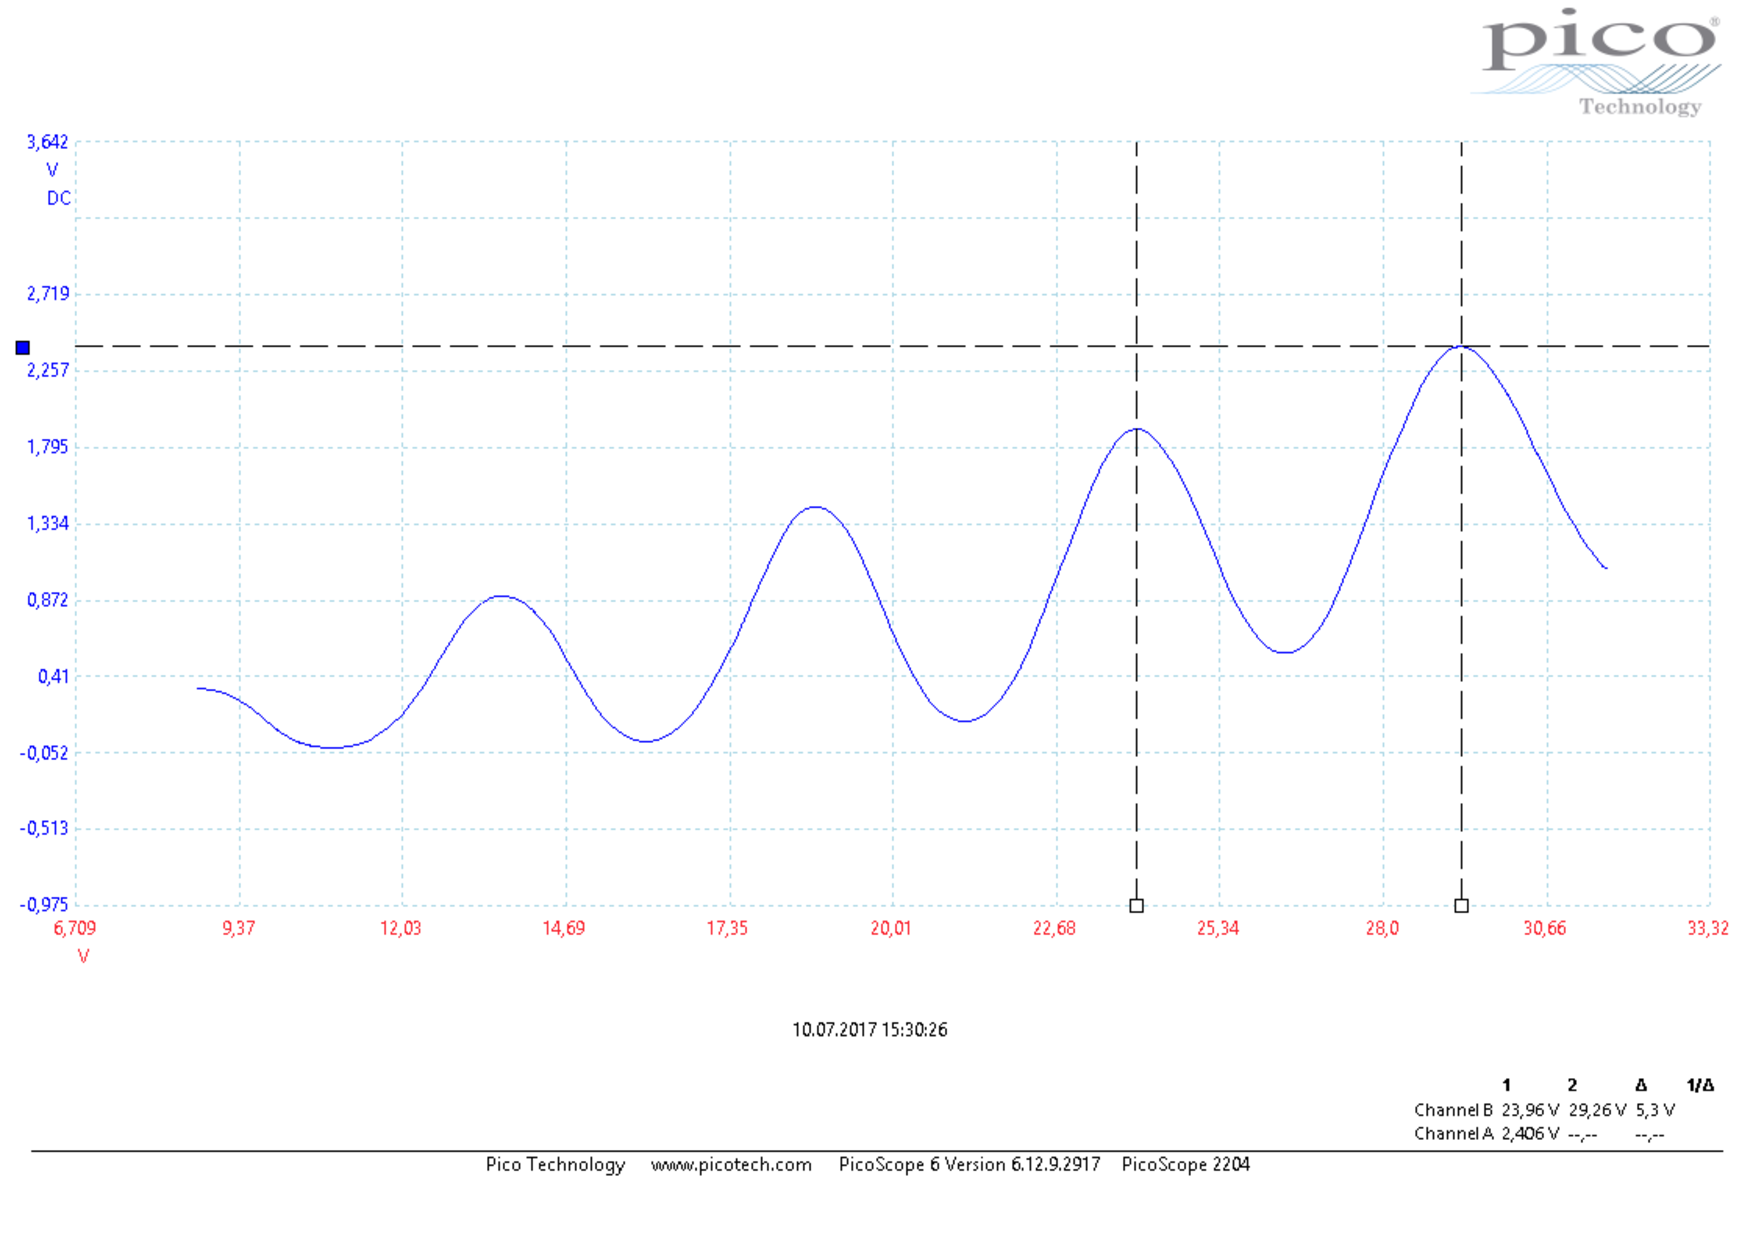
\includegraphics[width=\textwidth]{../Daten/Aufgabe1/Frank_Hertz_140.pdf}
	\caption{Graph bei 140$ ^\circ $C}
	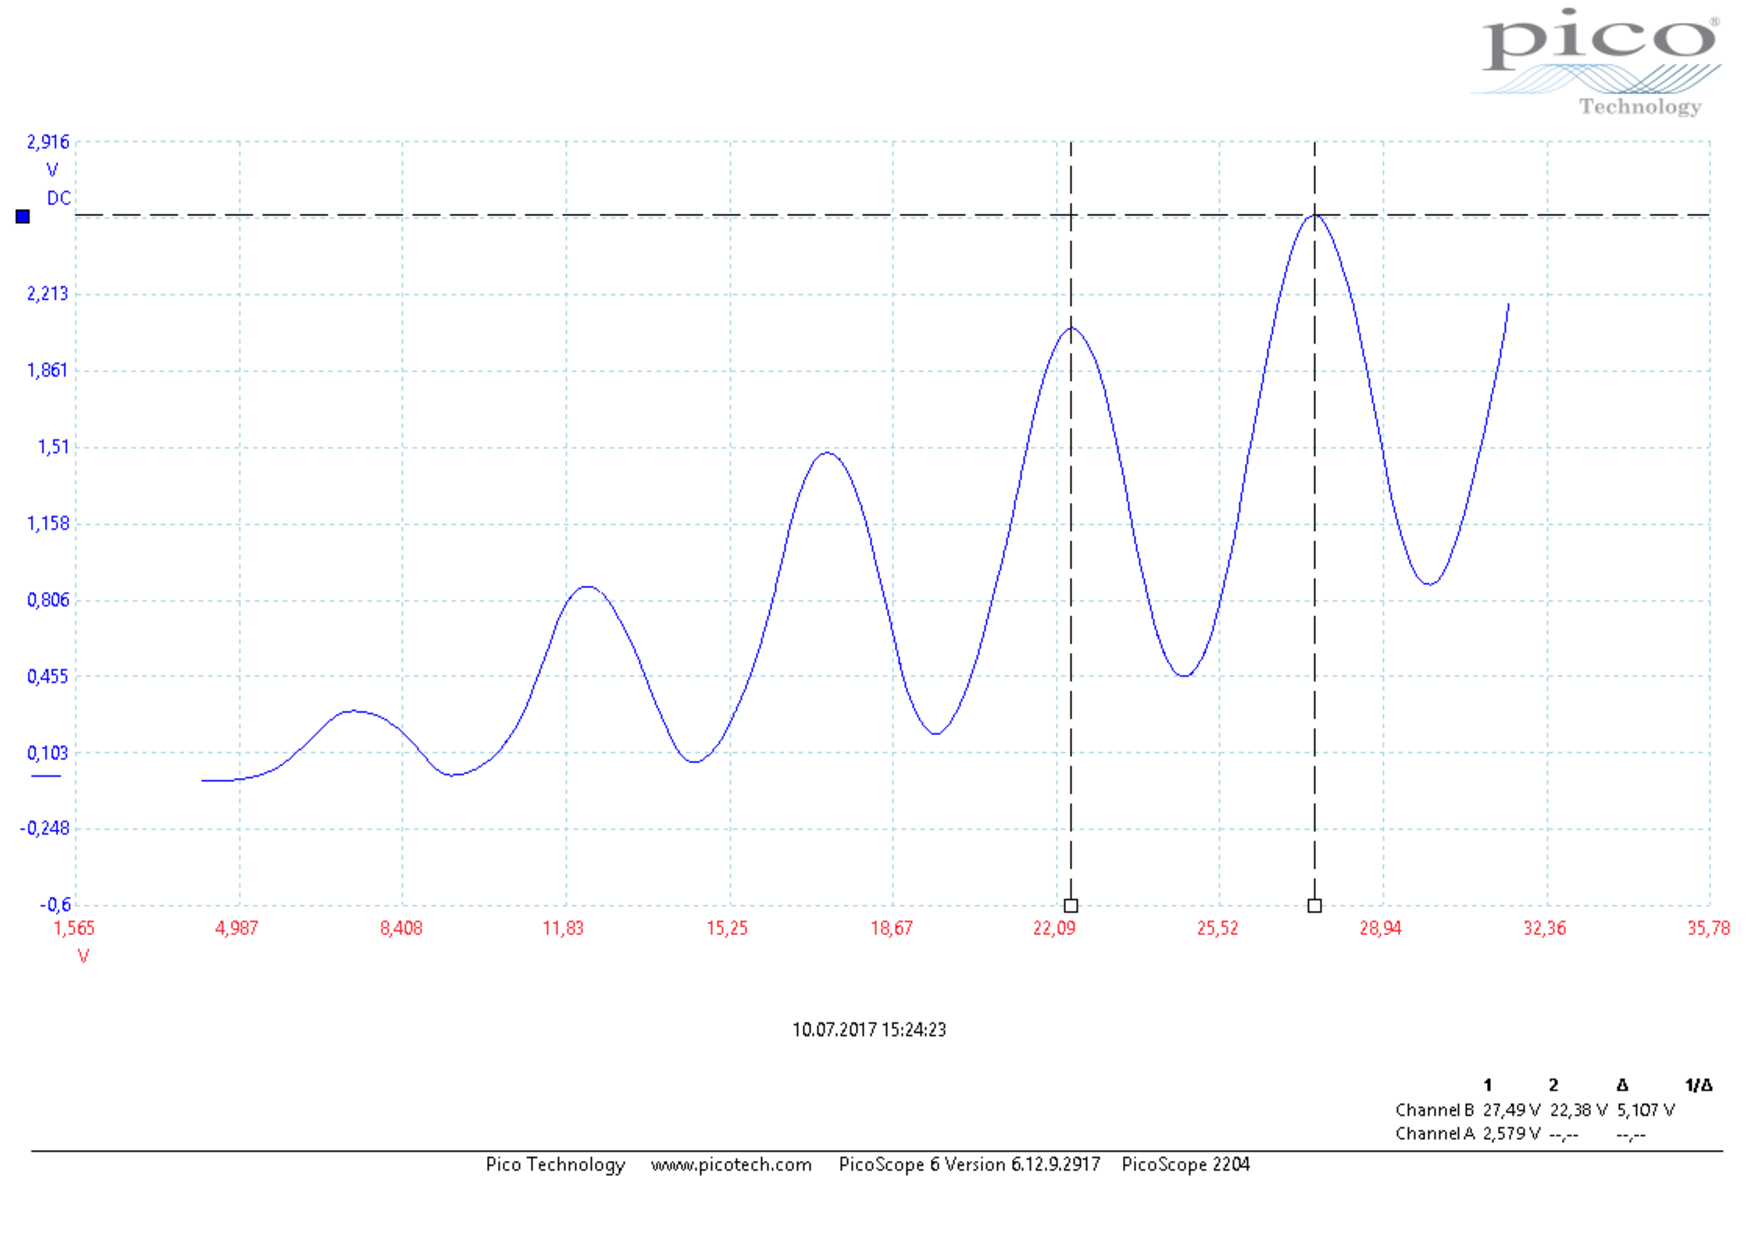
\includegraphics[width=\textwidth]{../Daten/Aufgabe1/Frank_Hertz_150.pdf}
	\caption{Graph bei 150$ ^\circ $C}
\end{figure}
\begin{figure}
	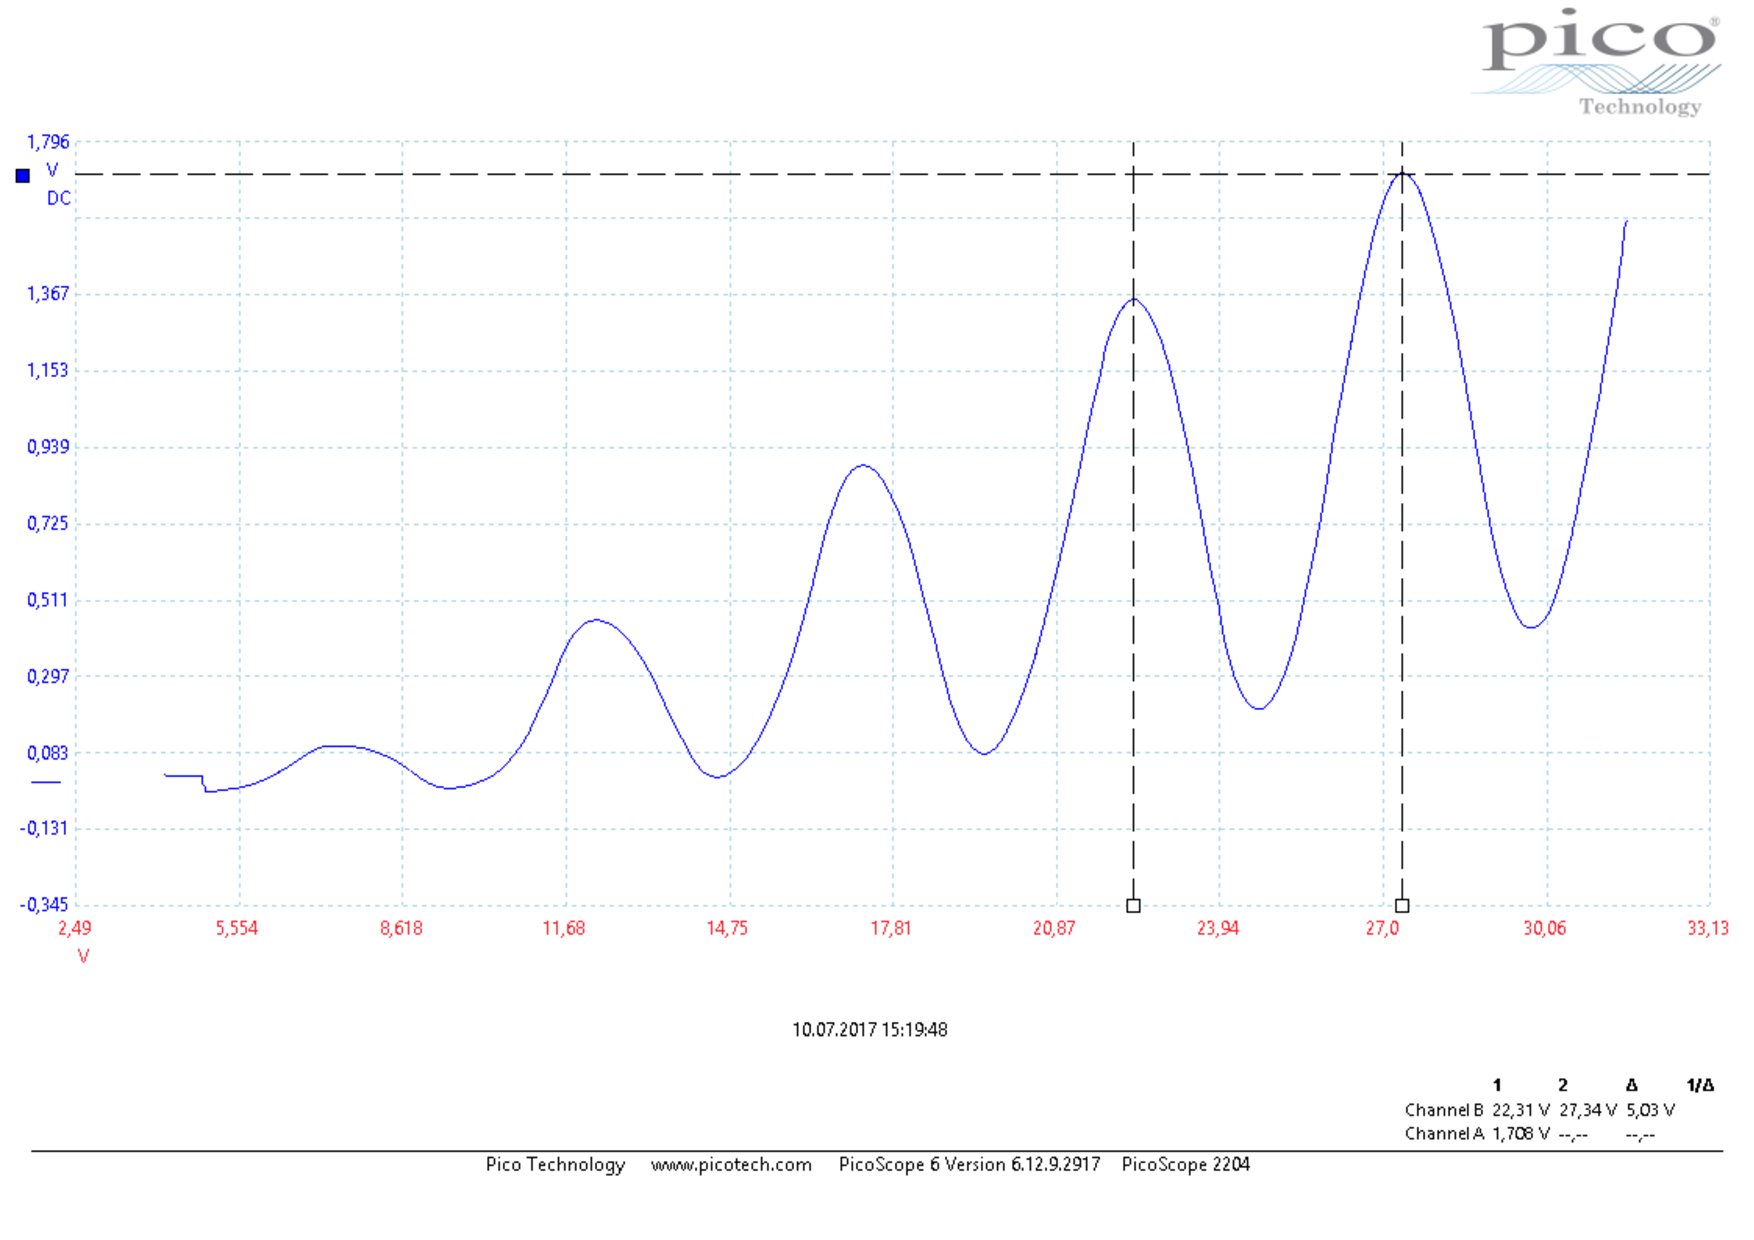
\includegraphics[width=\textwidth]{../Daten/Aufgabe1/Frank_Hertz_160.pdf}
	\caption{Graph bei 160$ ^\circ $C}
	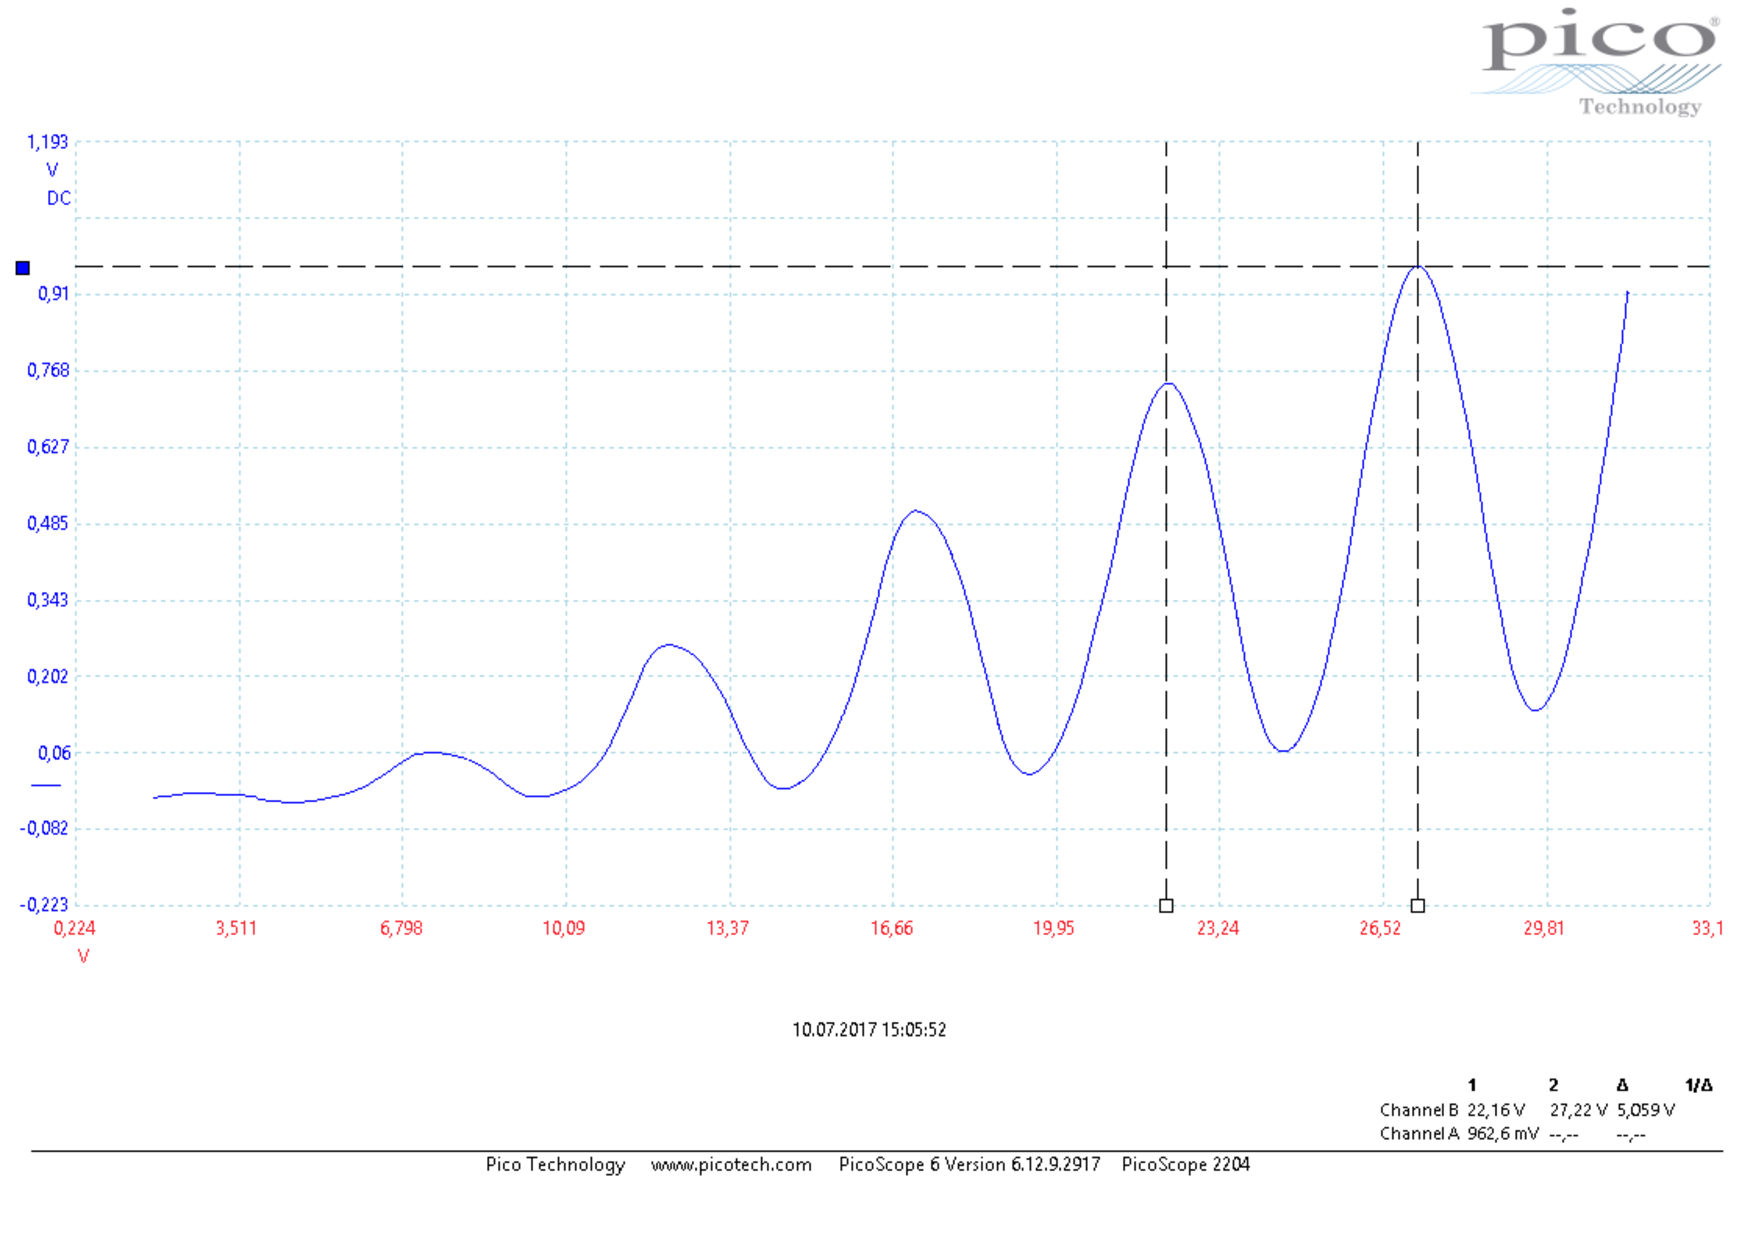
\includegraphics[width=\textwidth]{../Daten/Aufgabe1/Frank_Hertz_170.pdf}
	\caption{Graph bei 170$ ^\circ $C}
\end{figure}
\begin{center}
	\begin{tabular}{|c|c|c|c|c|c|c|}
		\hline
		T in $^\circ C$ & U$_1$ in V & U$_3$ in V & $\Delta U$ in V & $\Delta U$ in V & $\Delta U$ in V & $\Delta U$ in V \\ \hline
		170       &    3,94    &    1,17    &      4,793      &      4,971      &      5,06       &      5,001      \\ \hline
		160       &    3,94    &    1,17    &      4,882      &      5,001      &      5,006      &      5,03       \\ \hline
		150       &    3,94    &    1,17    &      4,906      &      4,983      &      5,113      &      5,107      \\ \hline
		140       &    3,0     &    2,26    &      4,942      &      5,092      &      5,232      &       5,3       \\ \hline
		120       &    1,98    &    2,71    &      5,134      &      5,232      &       5,3       &      5,729      \\ \hline
	\end{tabular} 
\end{center}
Somit erhalten wir die jeweiligen Thermospannungen über die Formel:
\begin{align*}
U_{Th}=U_{n}+U_{1}-n\cdot \overline{\Delta U}
\end{align*}
wobei $ \overline{\Delta U} $ der gemittelte Wert der $ \Delta U $ ist und $ U_{n} $ die Spannung des n-ten Peaks.
\begin{center}
	\begin{tabular}{|c|c|}
		\hline
		Temperatur in $^\circ$C & U$_{th}$ in V \\ \hline
		170           &     6,379     \\ \hline
		160           &     6,381     \\ \hline
		150           &     6,294     \\ \hline
		140           &     6,553     \\ \hline
		120           &     6,427     \\ \hline
	\end{tabular} 
\end{center}
Aus diesen Werten erhalten wir nun den gemittelten Wert $ \overline{U_{th}} =6,407\; $V.
\section{Das Raumladungsgesetz}
\begin{center}
	\begin{tabular}{|c|c|}
		\hline
		Spannung U$_2$ in V & Strom I$_{in}$ in nA \\ \hline
		0          &          0           \\ \hline
		1          &          0           \\ \hline
		2          &          0           \\ \hline
		3          &          0           \\ \hline
		4          &          10          \\ \hline
		5          &          10          \\ \hline
		6          &          20          \\ \hline
		7          &          20          \\ \hline
		8          &          30          \\ \hline
		9          &          30          \\ \hline
		10          &          40          \\ \hline
		11          &          40          \\ \hline
		12          &          50          \\ \hline
		13          &          60          \\ \hline
		14          &          60          \\ \hline
		15          &          60          \\ \hline
		16          &          70          \\ \hline
		17          &          70          \\ \hline
		18          &          80          \\ \hline
		19          &          80          \\ \hline
		20          &          90          \\ \hline
	\end{tabular} 
\end{center}
Nun überprüfen wir das Raumladungsgesetz bei einer Temperatur von 120 $ ^\circ $C. Wir erwarten einen Zusammenhang der Form $I\propto U_{2}^{3/2}  $, weswegen wir die Messdaten wie folgt fitten:
\begin{align*}
\log(I)=a\cdot \log(U_{2})+\log(b)
\end{align*}
\begin{figure}
	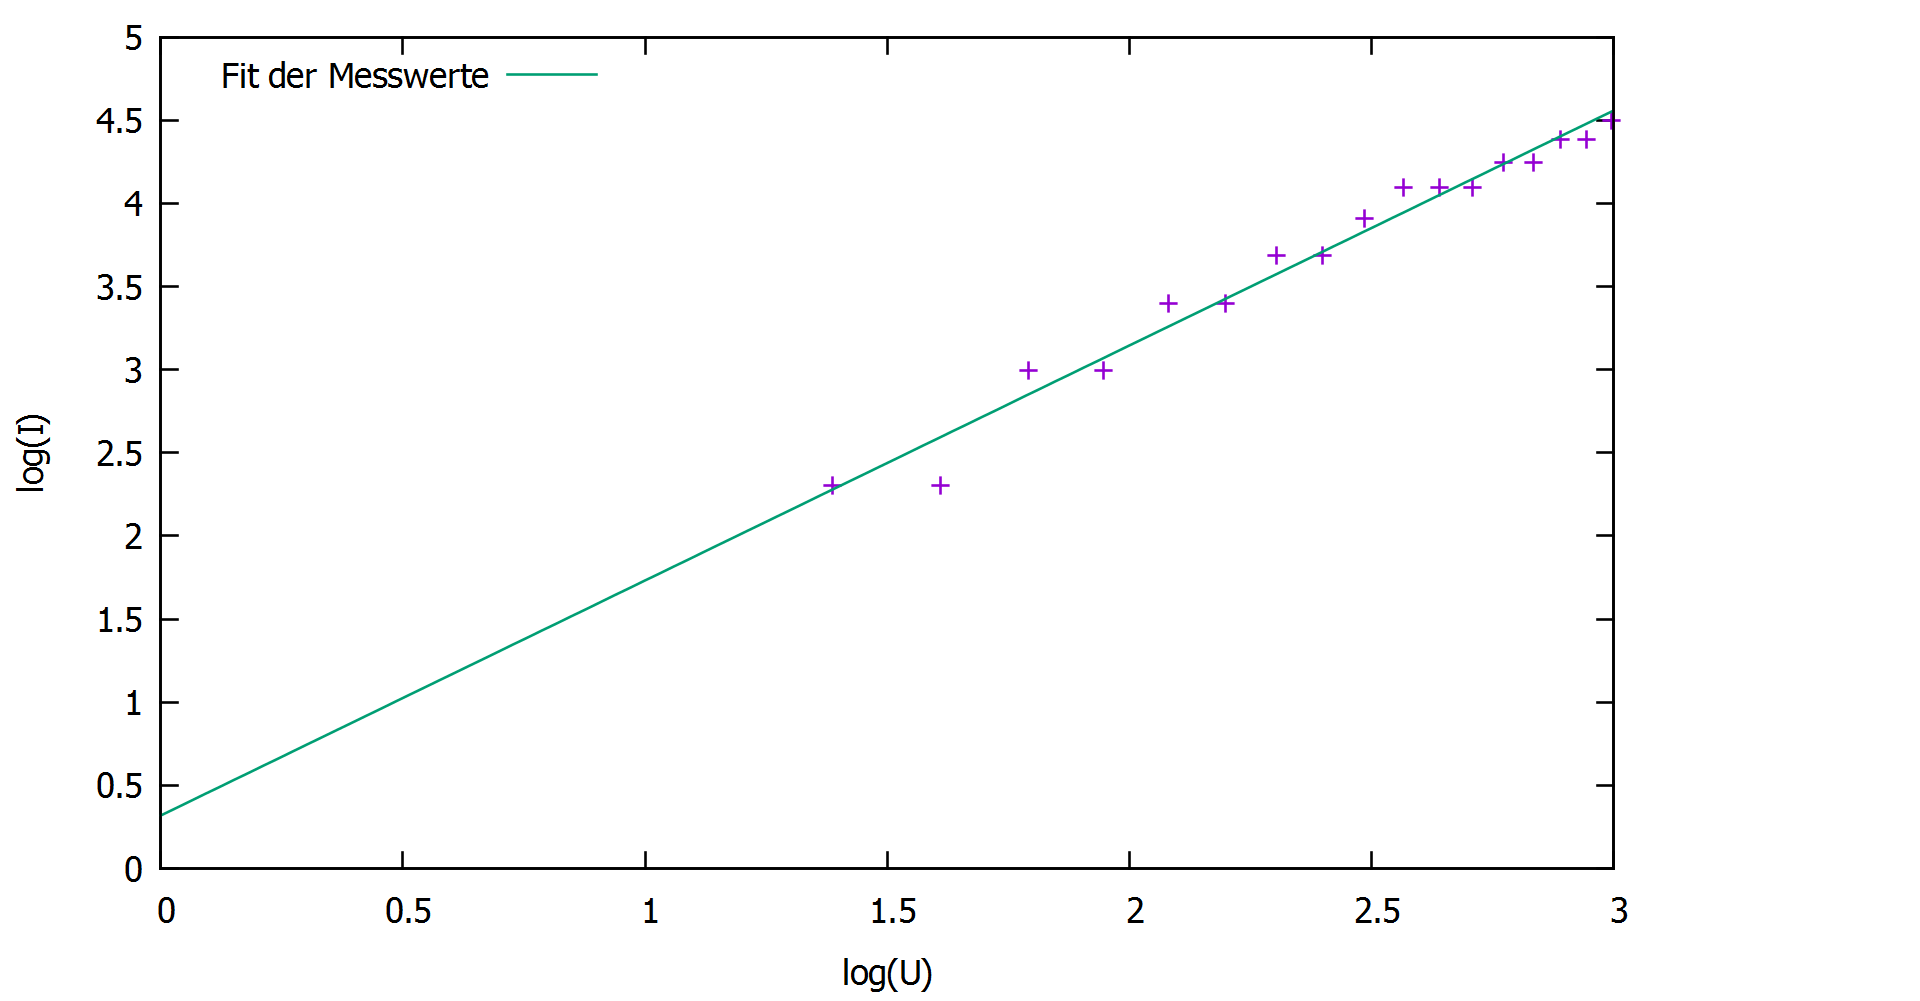
\includegraphics[width=\textwidth]{../Daten/Aufgabe1/Aufgabe1_3.png}
	\caption{Fit der Messwerte zu Aufgabe 1.3}
\end{figure}
Die mit Gnuplot erstellte Funktion hat die Steigung a=1,414. Vergleicht man dies mit dem erhofften Wert(1,5) erhält man einen Fehler von 5,7\%.
\begin{center}
	\begin{tabular}{|c|c|}
		\hline
		Spannung U$_2$ in V & Strom I$_{in}$ in nA \\ \hline
		0          &          0           \\ \hline
		1          &          0           \\ \hline
		2          &          0           \\ \hline
		3          &          0           \\ \hline
		4          &          10          \\ \hline
		5          &          10          \\ \hline
		6          &          20          \\ \hline
		7          &          20          \\ \hline
		8          &          30          \\ \hline
		9          &          30          \\ \hline
		10          &          40          \\ \hline
		11          &          40          \\ \hline
		12          &          50          \\ \hline
		13          &          60          \\ \hline
		14          &          60          \\ \hline
		15          &          60          \\ \hline
		16          &          70          \\ \hline
		17          &          70          \\ \hline
		18          &          80          \\ \hline
		19          &          80          \\ \hline
		20          &          90          \\ \hline
	\end{tabular} 
\end{center}
\section{Ionisationsarbeit}
Nun wollen wir die Ionisationsarbeit von Quecksilber bei 120 $ ^\circ $C bestimmen.
\subsection{Methode a}
Zunächst bestimmen wir die Ionisationsarbeit indem wir die Stromstärke I$ _{in} $ über die Spannung U$ _2 $ auftragen und zwei geraden durch die Messpunkte legen. Der Schnittpunkt der geraden beschreibt dann die Ionisationsarbeit. Hierbei stellt sich jedoch heraus, das einige Werte zu stark von der Form einer geraden abweichen, weswegen diese Messpunkte vernachlässigt wurden. 
\begin{figure}
	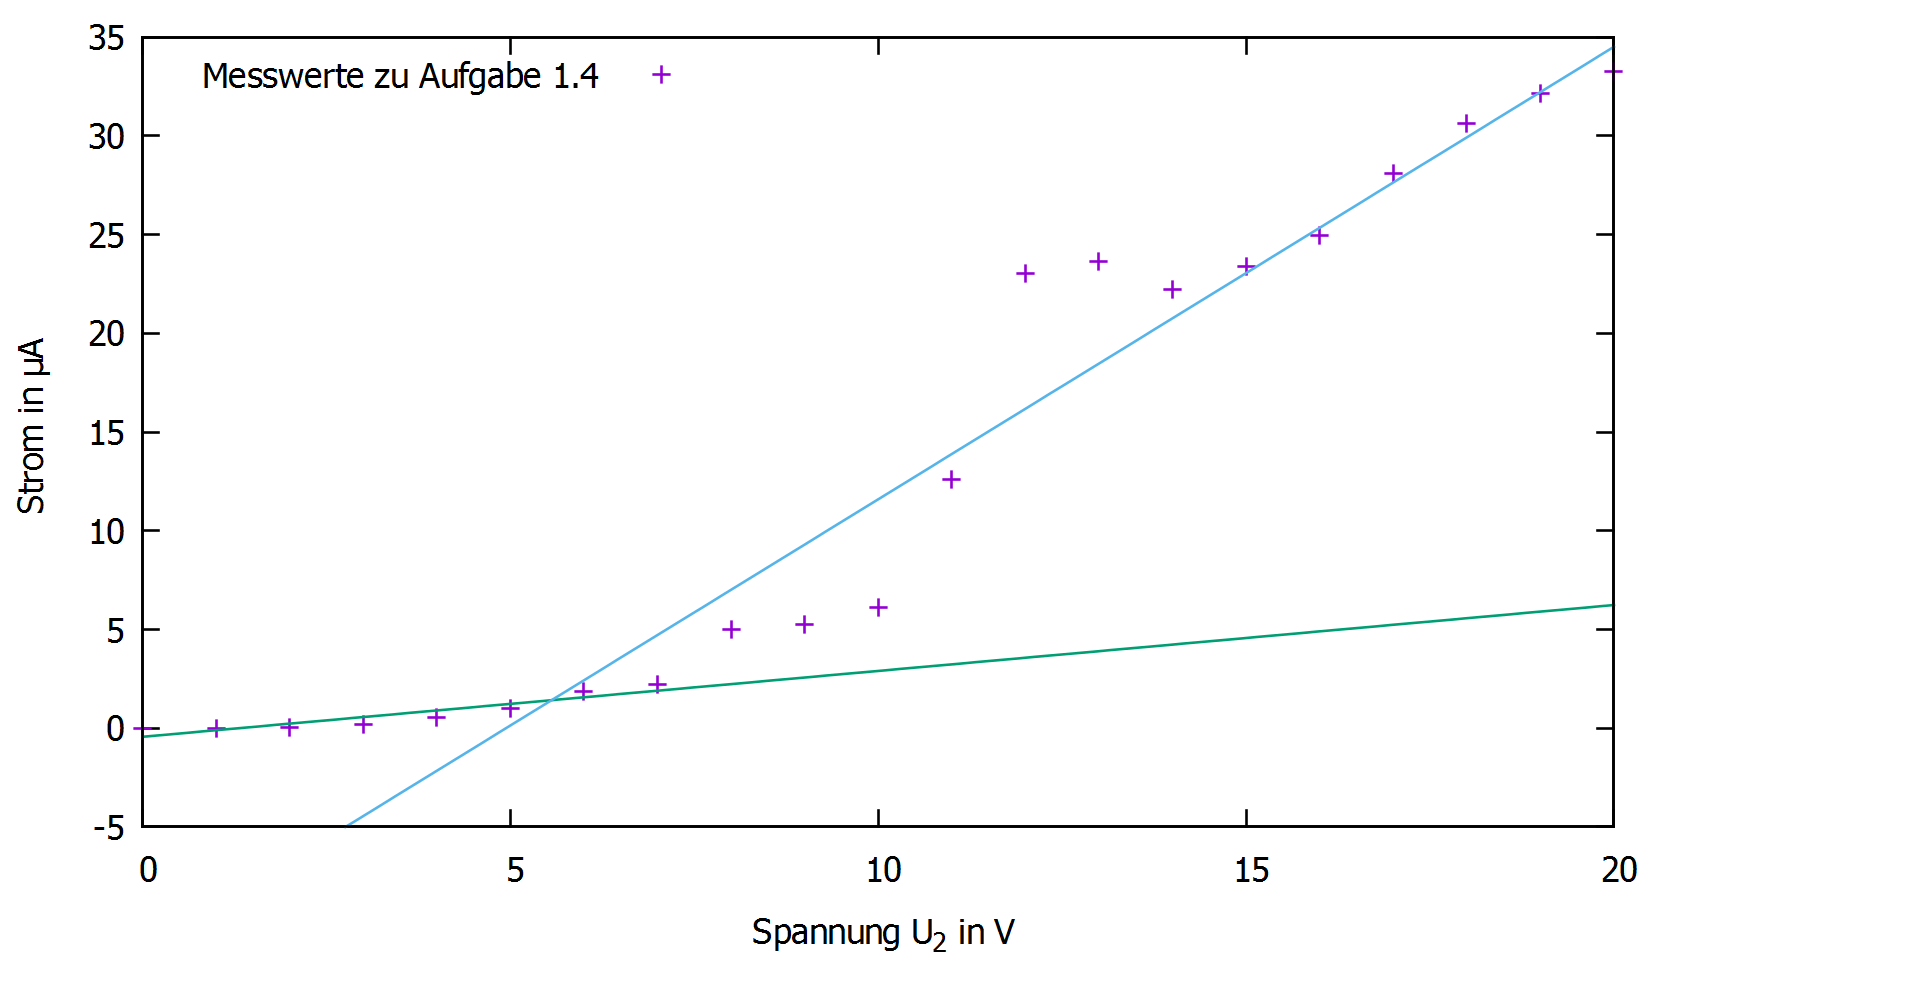
\includegraphics[width=\textwidth]{../Daten/Aufgabe1/Aufgabe1_4.png}
	\caption{Fit der Messwerte zu Aufgabe 1.4.a}
\end{figure}

Der Schnittpunkt befindet sich bei U$ _2 $= 5,579 V verrechnen wir nun noch die Thermokontaktspannung aus 1.1 erhalten wir die Ionisationsarbeit  11,986 eV. Dies entspricht einer Abweichung vom Literaturwert (10,44 eV) von 12,9\%. Wir vermuten, dass dieser Fehler aufgrund von nicht beachteten Umständen während der Versuchsdurchführung entstand, da die gemessenen Werte ebenfalls sehr ungewöhnlich aussehen.
\begin{center}
	\begin{tabular}{|c|c|}
		\hline
		Spannung U$_2$ in V & Strom I$_{in}$ in $\mu$A \\ \hline
		0          &            0             \\ \hline
		1          &           0,01           \\ \hline
		2          &           0,05           \\ \hline
		3          &           0,19           \\ \hline
		4          &           0,53           \\ \hline
		5          &           1,01           \\ \hline
		6          &           1,85           \\ \hline
		7          &           2,23           \\ \hline
		8          &           5,0            \\ \hline
		9          &           5,28           \\ \hline
		10          &           6,11           \\ \hline
		11          &          12,58           \\ \hline
		12          &          23,05           \\ \hline
		13          &          23,65           \\ \hline
		14          &          22,22           \\ \hline
		15          &           23,4           \\ \hline
		16          &          24,97           \\ \hline
		17          &          28,09           \\ \hline
		18          &          30,64           \\ \hline
		19          &          32,17           \\ \hline
		20          &          33,26           \\ \hline
	\end{tabular} 
\end{center}
\subsection{Methode b}
\begin{figure}
	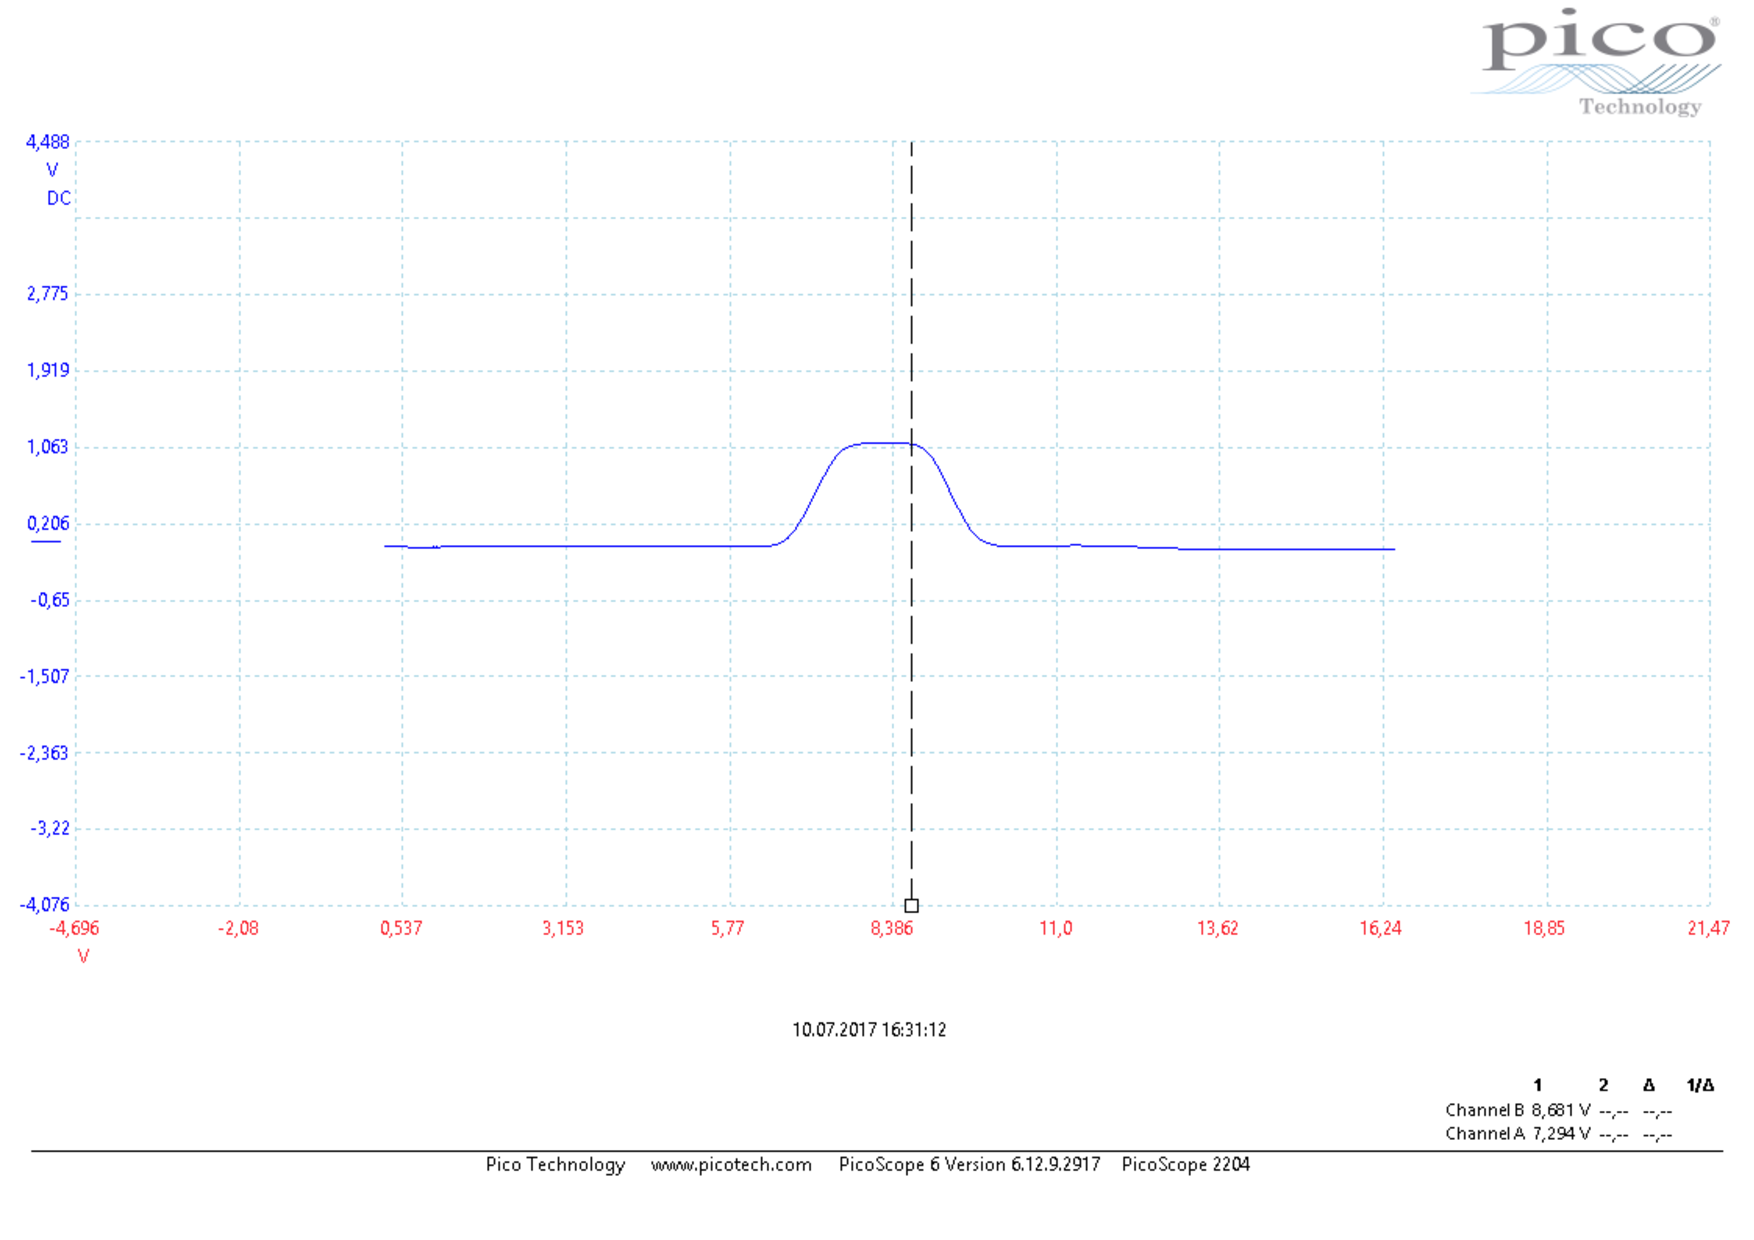
\includegraphics[width=\textwidth]{../Daten/Aufgabe1/Frank_Hertz_1_4_b_2.pdf}
	\caption{Graph zu Aufgabe 1.4.b}
\end{figure}
Als zweite Variante wurde die Spannung direkt aus dem Graphen abgelesen, wobei dieser ebenfalls Ungewöhnlich aussieht. Mit dieser Methode erhalten wir eine Ionisationsarbeit von 10,789 eV, was einem Fehler von 3,2\% entspricht.
\section{Emissionsspektrum der Gasentladung}
Als letztes betrachten wir die Gasentladung mithilfe eines Taschenspektroskops. Hierbei konnten wir die Farben Rot, Gelb, Grün und Lila erkennen. Es ist möglich, dass es noch weitere sichtbare Farben gab, die wegen angelassenem Raumlicht nicht erkennbar waren.